\documentclass[DIV=19,paper=A5,fontsize=10pt]{scrartcl}
%\documentclass[DIV=21,paper=20cm:20cm,9pt]{scrartcl}
\def\spal{2}
\setlength{\columnseprule}{0.4pt} % line between column

\usepackage{titlesec}
\usepackage{multicol}
\usepackage{lettrine}

\usepackage{dingbat}
\usepackage{collect}
\usepackage{ulem}
\definecollection{trs}

%\usepackage[hidelinks]{hyperref}
\usepackage{cleveref}
%\hypersetup{
%pdftitle={Pentagame Regulae Rules Regeln Regles},
%pdfsubject={Pentagame Rules in Many Languages},
%pdfauthor={Jan Suchanek et al.},
%pdfkeywords={Pentagame board game rules explained latin english german deutsch latine francais russian chinese spanish espaniol}
%}


\usepackage[dvipsnames]{xcolor}
\usepackage{tikzpeople}

\usepackage{framed}
\usepackage{polyglossia}
\usepackage{xeCJK}
\providecommand{\chapterformat}{}
\setmainlanguage{english}
\setotherlanguages{french,ngerman,latin,bahasai,russian,greek,spanish,georgian,swedish,polish,danish,arabic}

\DeclareTextCommandDefault{\cyrdash}{\hbox to.8em{---}~}

\makeatletter
\newcommand\footnoteref[1]{\protected@xdef\@thefnmark{\ref{#1}}\@footnotemark}
\makeatother

\newCJKfontfamily{\tradChinesefont}{AR PL UKai HK}[BoldFont=Noto Sans CJK TC Bold]
\newfontfamily\arabicfont[Script=Arabic]{Amiri}
\newfontfamily\arabicfontsf[Script=Arabic]{Amiri}

\usepackage{setspace}


\usepackage{microtype}


% does not seem necessary at all?!
%\setmainfont{FreeSans}
\setsansfont{FreeSans}
\setmainfont{FreeSerif}
\setmonofont{FreeSerif}

\usepackage{tikz}
\raggedbottom
\raggedcolumns
\clubpenalty = 10000
\widowpenalty = 10000
\displaywidowpenalty = 10000

\newcommand{\noun}[1]{\textsc{#1}}

\newcounter{oldpage}

\makeatletter
\renewcommand\paragraph{%
\@startsection{paragraph}{4}%
{\z@}{1ex\@plus 1ex \@minus .2ex}%
{0.2ex \@plus .2ex}%
  {\sffamily\normalsize\bfseries}%
 }
 \makeatother

%%% Document specific commands

\newcommand{\myskip}{\smallskip}
\newcommand{\headline}{{\LARGE{}Pentagame}}
\newcommand{\tocent}{}
\newcommand{\translator}{}
\newcommand{\general}{}
\newcommand{\choosext}{}
\newcommand{\choosex}{}
\newcommand{\setupt}{}
\newcommand{\setup}{}
\newcommand{\objectivet}{}
\newcommand{\objective}{}
\newcommand{\rulest}{}
\newcommand{\rules}{}
\newcommand{\website}{\textsf{\textbf{pentagame.org}}}
\newcommand{\myhead}{\begin{centering}{\sffamily\Large{\textbf\headline}}\end{centering}}


%%% THE ACTUAL LAYOUT %%%
\newcommand{\layout}{
    \begin{framed}
        \centering {{{\Large{\textbf{\tocent}}}}}
    \end{framed}
    \addcontentsline{toc}{section}{\tocent}
    \begin{multicols}{2}
    \general
    \paragraph*{\choosext}
    \choosex
    \paragraph*{\setupt}
    \setup
    \paragraph*{\objectivet}
    \objective
    \paragraph*{\rulest}
    \rules
    \par
    %\hfill{\footnotesize{(\translator)}}
    \end{multicols}
    \newpage
}

\newcommand{\layoutara}{
    \begin{framed}
        \centering {{{\LARGE{\textbf{\tocent}}}}}
    \end{framed}
    \addcontentsline{toc}{section}{\tocent}
    \begin{multicols}{2}
    \RLmulticolcolumns
    
        \general
        
        \medskip\uline{\textbf{\choosext}}\smallskip
        
        \choosex
        
        \medskip\uline{\textbf{\setupt}}\smallskip
        
        \setup
        
        \medskip\uline{\textbf{\objectivet}}\smallskip
           
        \objective
        
        \medskip\uline{\textbf{\rulest}}\smallskip
        
        \rules
        
    %\hfill{\footnotesize{(\translator)}}
    \end{multicols}
    \newpage
}

\setlength{\parskip}{0ex}
\setlength{\parindent}{0cm}


\title{Penta$\cdot$game: The Rules in Text}
%\subtitle{The diceless pentagram shaped board game}
\author{by Jan Suchanek}
\publishers{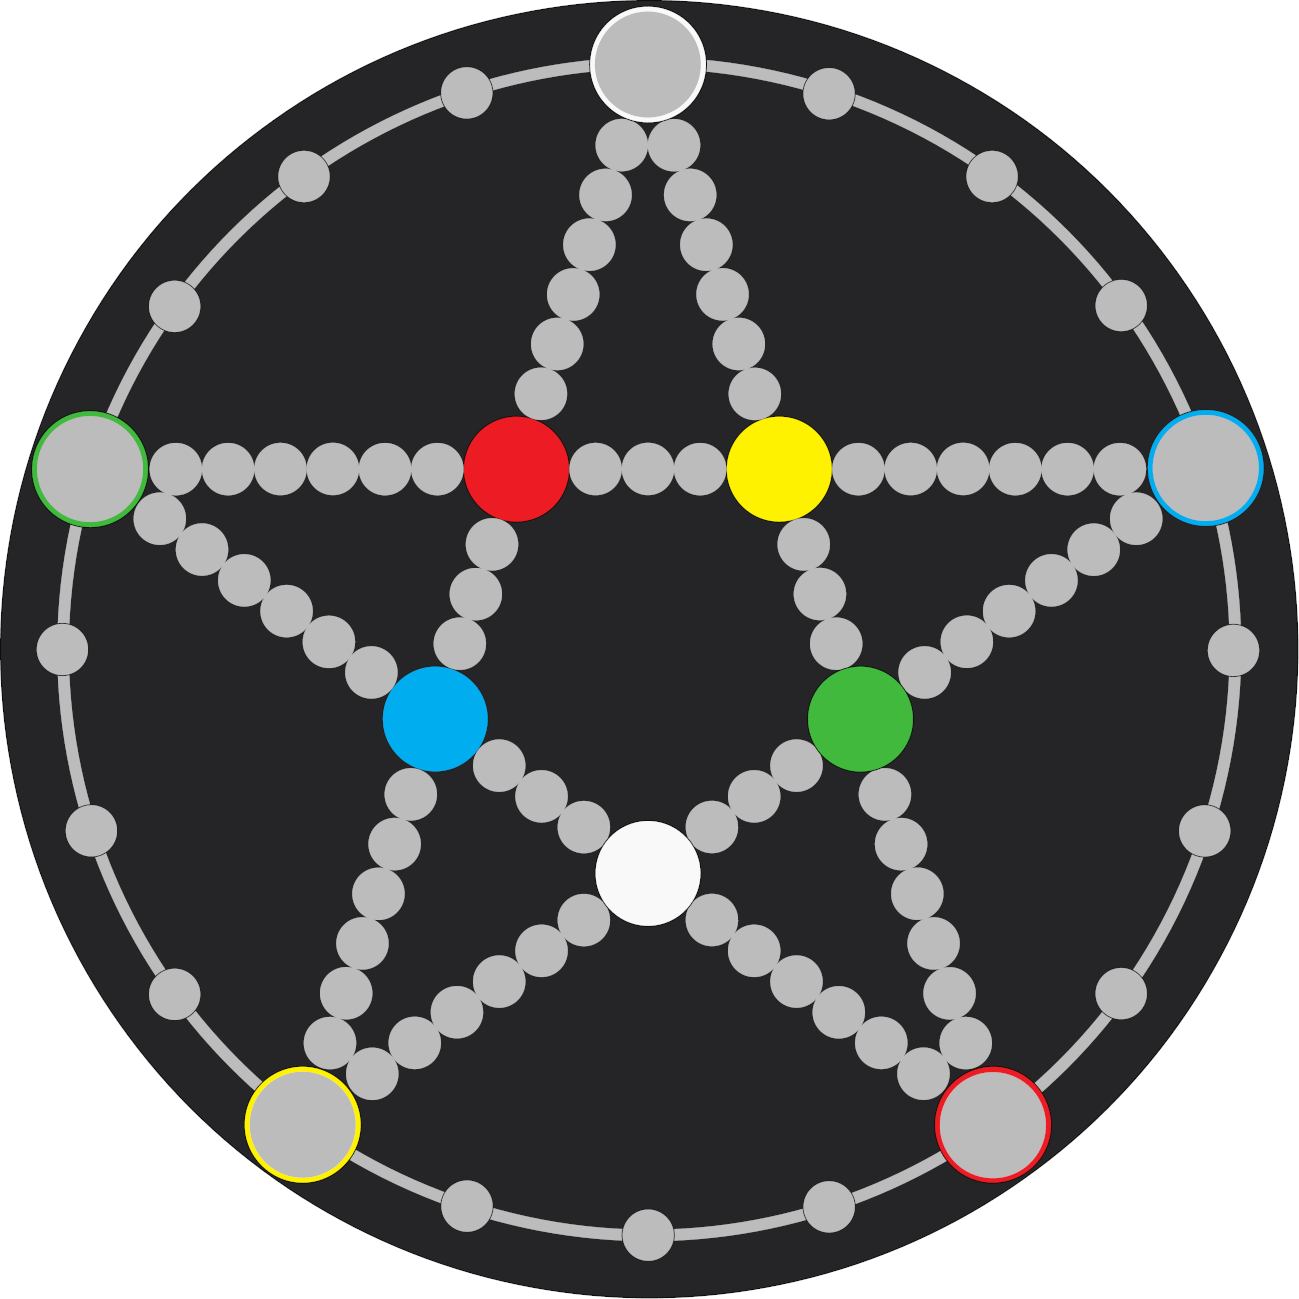
\includegraphics[width=0.5\textwidth]{Pentagame-board-nob.png}}
\date{}

%% Actual Document. Calling the content first, then printing the same layout.

\begin{document}

\maketitle

\setlength\columnsep{50pt}
\begin{multicols}{2}
\makeatletter
\renewcommand\tableofcontents{%
    \@starttoc{toc}%
}
\makeatother
\tableofcontents
\end{multicols}
\setlength\columnsep{10pt}

\newpage



\begin{otherlanguage}{latin}
    \renewcommand{\headline}{Penta$\cdot$ludus - Latine}
\renewcommand{\tocent}{Latine}
\renewcommand{\translator}{Dr.~J\"org Grimm, JS}
\renewcommand{\general}{ 

%\textbf{Descriptio }
\lettrine[lines=3]{L}{udus}
mirabilis atque explicabilis velox. 
Duo lusores ludent tertia pars horae, tres aut quattuor ludent hora. 

Aela non opus est. 
Aptus ab quinque anni lusoris.
Tabula pentagrammiforma, quattuor cohortes quinorum peditum coloratorum, quina impedimenta nigra et cana Penta\-ludum componunt.  Fit Ioh.~\noun{Aridus.}


%\textbf{Cohortes }





}
\renewcommand{\choosext}{Cohortes}
\renewcommand{\choosex}{
Lusor quisque agit pedites quinos, quibus est eadem forma (aut stella aut luna \&c.), sed sunt diversi colores. 

Sic tua cohors peditem caeruleum, peditem rubrum  \&c. continet.

}

\renewcommand{\setupt}{Dispositio} 
\renewcommand{\setup}{ 
In quinque nodis positis in circulo, qui circumvenit pentagramma, ponite pedites eiusdem coloris: pedites albos in nodo albo, caeruleos
in nodo caeruleo \&c. 

Praeter illa decem loca quae nodos formant, existunt alter octoginta aedicula in viis, ubi pedites in ludo etiam possunt collocari. 

Sunt etiam impedimenta nigri et im\-pe\-di\-men\-ta cana. 

Impedimenta nigra ponite in nodis centri. In centro retinete impedimenta cana. 
}

\renewcommand{\objectivet}{Propositum} 
\renewcommand{\objective}{ 

Destinatio per unum quemque peditem, qui occupat nodum externi circuli, est nodus eiusdem coloris in interno pentagrammatis. 
Albo est eundum ad album, rubro ad rubrum \&c. 

Lusor victor qui duxit tres pedites ad nodum aequi coloris.

}

\renewcommand{\rulest}{Regulae } 
\renewcommand{\rules}{ 
Duc peditum tuorum unum in quamvis directionem sequens aut viam circuli aut vias stellae, quoad per regulas potes occupare aediculum. 

\myskip

In quodlibet aediculo libero, ubi  duae lineae conveniunt, tibi licet de via recta declinare sine retentione. 

\myskip

At numquam tibi licet transcendere nec impedimenta nec pedites alios.

\myskip

Potes vero ingredi in aediculum occupatum:

\myskip

Se ibi stat impedimentum nigrum, id pone in aediculo libero ad libitum. 

Se ibi iam stat pedes alius, pedites positiones suas mutare debent.

Se ibi sunt plures pedites (non potest fieri, nisi initio ludi), elige unum mutandum.

\myskip

Ita potes etiam mutare positiones duorum peditum tuorum.



\myskip


Bis eundem ne cana; eundem motum non licet iterum.

\myskip

Pedes progressus ad finem ludo abit. Pone eum in centrum.

Accipe per illo impedimentum canum et colloca in aediculo, quoad tibi paret. 

\myskip

Quando captas tale impedimentum canum, remove a tabula.

\myskip

Pedes ponetus ad finem per aliter lusor  deinde iacet abitere.

\myskip

Peragitur orbis ultimus.% ad finem ludetur.
%Lusor  qui primus tres pedites ad finem duxit ludo victor.
}

    \layout 
\end{otherlanguage}

\begin{otherlanguage}{spanish}
    
\renewcommand{\headline}{Penta$\cdot$juego - Español}	
\renewcommand{\tocent}{Español}	
\renewcommand{\translator}{Juan José Bravo / Carlos Ayon}	
\renewcommand{\general}{
    \lettrine[lines=3]{U}{n}
    juego que se explica en un minuto, pero que sigue fascinándote durante años. 
    Una partida entre dos jugadores puede llevarte 20 minutos. Tres o cuatro jugadores pueden tardar hasta 90 minutos.	
    Se juega sin dados. Apto para todos, a partir de los cinco años.	
    En la caja: 4 x 5 figuras de colores, 5 bloques negros, 5 grises y un tablero.	
}		
	
\renewcommand{\choosext}{Elije tus figuras}	
\renewcommand{\choosex}{	
En la caja hay un grupo de figuras por jugador.Cada equipo esta compuesto por cinco figuras; una azul, una roja, una blanca, una verde  y una amarilla.	
Las figuras se colocan en los círculos exteriores de los colores correspondientes:
Ellas tendrán que llegar a la meta situada en el medio del tablero. 	
}	

\renewcommand{\setupt}{Instalación}	
\renewcommand{\setup}{	
Disponed vuestras figuras sobre los círculos exteriores en sus colores correspondientes: 
la figura blanca en el circulo exterior blanco, la azul en circulo exterior azul, etc.	
	
Dispón los bloques negros en los cinco círculos interiores en el medio del tablero.
Coloca los bloques grises en el centro del tablero.	
}	
	
\renewcommand{\objectivet}{Objetivo}	
\renewcommand{\objective}{	
Las figuras blancas deben alcanzar los círculos interiores blancos, las figuras azules los círculos interiores azules, etc.	
El destino es siempre el gran circulo central, del color correspondiente a la figura, en el medio del pentagono opuesto al punto de partida.	
	
Coloca \emph{tres} de tus cinco peones en los círculos de colores correspondientes para ganar.
}	
	
\renewcommand{\rulest}{Reglas del juego}	
\renewcommand{\rules}{	
Mueve la figura de tu elección sobre el tablero de juego sin importar la dirección, tan lejos como quieras.	
	
Puedes girar en cualquier esquina o interseccion libres, sin detenerte.	
	
No podrás saltar sobre ningun bloque o figura, pero podrás colocarte en un circulo  ocupado:	
	
\myskip	
	
Si caes en un circulo ocupado por un bloque negro, tomalo y colocalo en cualquier espacio libre de tu elección.	
	
Si caes en un circulo ocupado por otra figura, intercambia tu lugar anterior con ella.	
	
	
Puedes cambiar de posición entre dos peones de tu propio equipo. 	


Si caes en una casilla ocupada por varias figuras, puedes elegir una de ellas e intercambiar de lugar.	

\myskip	
	
No puedes hacer el mismo movimiento dos veces seguidas.	

\myskip
	
Cuando una figura llega a su meta, es retirada del juego. Se le coloca en el centro del tablero y se toma un peón gris que podrás colocar en cualquier circulo libre de tu elección.
	
\myskip		
	
Si caes en un lugar ocupado por un bloque gris, este sera retirado del juego nuevamente.	

\myskip	

Si otro jugador te ha movido hacia tu meta, debes avanzar a ella una vez que sea tu turno.

\myskip	

La última ronda se juega hasta el final.
	
% El primer jugador que consiga retirar tres de sus figuras ganará la partida.%
}


    \layout
\end{otherlanguage}

\begin{otherlanguage}{french}
    \renewcommand{\headline}{Penta$\cdot$jeux - Fran\c{c}ais}
\renewcommand{\tocent}{Fran\c{c}ais}
\renewcommand{\translator}{Armelle Journaix}
\renewcommand{\general}{ 
Un jeu de société qui s'explique en une minute mais reste fascinant pendant des années.

À deux, la partie dure environ 20 minutes. 
À trois ou quatre, la partie peut durer jusqu'à 90 minutes.

Aucun dé requis.
Âge : à partir de 5 ans. 
Par Jan \noun{Suchanek}.

Contenu de la boîte : 4 familles de 5 pions en couleurs, 5 pions noirs, 5 pions gris, un plateau.

}
\renewcommand{\choosext}{Choisissez vos pions}
\renewcommand{\choosex}{
Chaque joueur dispose de cinq pions.
Une famille est composée de cinq pions et il y en a cinq par joueur dans la boîte.

%Il y a la famille aux cheveux argentés, la famille aux cheveux noirs, une famille aux cheveux dorés et une famille chauve.

Chaque équipe est composée de cinq pions : un bleu, un rouge, un blanc, un vert et un jaune.
}

\renewcommand{\setupt}{Installation}
\renewcommand{\setup}{ 
Disposez vos pions sur les cercles extérieurs correspondant aux couleurs des pions : votre pion blanc sur le cercle extérieur blanc, votre pion bleu sur le cercle extérieur bleu, etc.

Disposez les pions noirs sur les cercles intérieurs en couleurs.

Posez les pions gris au centre du plateau de jeu.
}

\renewcommand{\objectivet}{But du jeu}
\renewcommand{\objective}{
Les pions blancs doivent se rendre sur le cercle intérieur blanc, les pions bleus sur le cercle intérieur bleu, etc.

Le but est toujours le cercle intérieur coloré à l'opposé du cercle de départ.

Soyez le premier à déplacer trois de vos cinq pions sur leurs cercles intérieurs colorés respectifs pour gagner.
}

\renewcommand{\rulest}{Règles du jeu}
\renewcommand{\rules}{
Déplacez le pion de votre choix sur le plateau de jeu, où vous voulez et dans n'importe quelle direction.

Vous pouvez utiliser tous les chemins possibles.

Vous ne pouvez pas sauter les cercles occupés par des pions, quelle que soit leur couleur.

\myskip

Mais vous pouvez poser votre pion sur un cercle déjà occupé :

\myskip

Si vous posez votre pion sur un cercle occupé par un pion noir, prenez le pion noir et posez-le ensuite où vous voulez sur un cercle libre.

Si vous déplacez votre pion sur un cercle occupé par un autre pion, vous changez de place avec lui.

\myskip

Vous pouvez changer de place entre deux pions de votre famille.

Si vous déplacez votre pion sur une case occupée par plusieurs autres pions, choisissez-en un et changez de place avec lui.

\myskip

Vous ne pouvez pas effectuer le même déplacement deux fois de suite.

\myskip

Un pion qui atteint son but est retiré du jeu.

Ensuite, prenez l'un des pions gris du centre du jeu et placez-le sur le cercle de votre choix.

Si votre pion se pose à la place d'un pion gris, le pion gris est retiré du jeu.

\myskip

Si un autre joueur vous a déplacé vers votre but, vous devez partir une fois que c'est votre tour.


\myskip

Le %premier 
joueur qui retire trois de ses pions du plateau gagne la partie.%
}
    \layout
\end{otherlanguage}

\begin{otherlanguage}{ngerman}
    \selectlanguage{ngerman}
\renewcommand{\headline}{Penta$\cdot$spiel - Deutsch}
\renewcommand{\tocent}{Deutsch}
\renewcommand{\translator}{J.S.}
\renewcommand{\general}{
\lettrine[lines=3]{E}{in} Spiel, das man in einer Minute begreift, das aber jahrelang fasziniert. 
Zu zweit dauert die Partie nur 20 Minuten. Drei oder vier Spieler spielen 40-90 Minuten.

Es gibt keine Würfel. Geeignet für Spieler ab 5 Jahren. Ein Spiel von Jan  \noun{Suchanek.}

In der Schachtel: 4$\times$5 farbige Figuren, 5 schwarze und 5 graue Blöcke und das Spielbrett.
}

\renewcommand{\choosext}{Figuren}
\renewcommand{\choosex}{
Jeder Spieler führt eine Mannschaft von fünf Figuren einer Form.
Jeder sucht sich eine Mann\-schaft aus.

In jeder solchen Mannschaft ist   eine blaue, eine rote, eine weiße, eine grüne und eine gelbe Figur.

Diese laufen alle von den fünf Ecken zu den fünf Kreuzungen, wo sie herausziehen.
}

\renewcommand{\setupt}{Aufbau}
\renewcommand{\setup}{
Stellt die Figuren geordnet nach Farben auf die fünf Ecken auf dem Kreis: die weißen auf das weiße Eckfeld, die blauen auf das blaue usw.

Je ein schwarzer Block kommt auf die Kreuzungen in der Mitte.

Die grauen Blöcke bleiben erst mal im Zentrum.
}

\renewcommand{\objectivet}{Ziel des Spiels}
\renewcommand{\objective}{
Weiße Figuren möchten zu der weißen Kreuzung, blaue zur blauen usw. 
Vom Rand her ist das Ziel immer die Kreuzung gleicher Farbe gegenüber.

Wer zuerst \emph{drei} seiner Figuren auf ihre jeweiligen Ziele zieht, gewinnt.
}

\renewcommand{\rulest}{Spielregeln}
\renewcommand{\rules}{
Ziehe eine deiner Figuren auf Stern oder Kreis in beliebiger Richtung beliebig weit.

Du kannst dabei an jeder freien Kreuzung ohne anzuhalten abbiegen.

Du darfst ziehen, aber nicht springen! Weder über Blöcke noch über andere Figuren!

\myskip

Jedoch kannst du auf ein Feld ziehen, das besetzt ist, und schlagen:

\myskip

Schlägst du einen schwarzen Block, so setze ihn auf ein beliebiges freies Feld. 

Schlägst du eine andere Spielfigur, so tauschen deine und diese Figur ihre Positionen.

\myskip

Auf diese Weise kann man zwei seiner eigenen Figuren vertauschen.

Ziehst du auf ein Feld, auf dem noch mehrere Figuren stehen, musst du mit \emph{einer }von ihnen tauschen.


 
\myskip 
 
Man darf nicht denselben Zug zweimal machen. 

\myskip 

Hat eine Figur ihr Ziel erreicht, so zieht sie raus. Sie kommt ins Zentrum. Dafür darf man von dort einen grauen Block ins Brett auf ein freies Feld setzen.

Schlägt man so einen grauen Block, so kommt er wieder raus.

\myskip 

Wirst du von einem anderen Spieler auf dein Ziel gebracht, so \emph{musst }du raus ziehen, sobald du dran bist.

\myskip

Die letzte Runde wird zu Ende gespielt.

% Wer zuerst  \emph{drei }seiner Figuren herauszieht, gewinnt.%
}
    \layout
\end{otherlanguage}

\begin{otherlanguage}{german}
    \renewcommand{\headline}{Penta$\cdot$speel - Platt}
\renewcommand{\tocent}{Plattdüütsch}
\renewcommand{\translator}{J.S.}
\renewcommand{\general}{
Kannst in een Minuut spitz\-kriegen liekers bleevt johrelang smakelk.

Twee Speler broken blots 20 Minuten. Dree or veer speeln 40-99 Minuten.

Wörpel gifft dat nich. Passlich för Speler af 5 Johren. En Speel vun Jan \noun{Suchanek}.

In de Lood: 4$\times$5 farvige Poppen, 5 swatte un 5 griese Blöck un de Speelbrett.
}

\renewcommand{\choosext}{Poppen}
\renewcommand{\choosex}{
Elk Speler föhrt en Koppel vun fief Poppen.

Jedereen söökt en so'n Koppel ut. 

In jede Koppel is 'ne blage, 'ne roote, 'ne witte, 'ne grööne un 'ne geele Popp. 

De trekken all vun de fief Ecken to de fief Krüüzen, wo se uttrekken. 
}

\renewcommand{\setupt}{Opbuu}
\renewcommand{\setup}{

Stellt de Poppen no Forben ordnet op de fief Ecken op de Krink: de witten op de witte Eck, de blage op de blaage, usw. 

Op jedereen Krüüz kummt en swatte Block.

De griesen bleven iersmol in de Midd. 
}

\renewcommand{\objectivet}{Teel vun de Speel}
\renewcommand{\objective}{
Witte Poppen wulln to dat witte Krüüz, blaage to dat blaage, usw. 

Vun de Krink her is de Teel ümmer de Krüüz mit de sülve Farve op de günt siet. 

Welkeen toeerst \emph{dree} vun sünne Poppen op de rechte Teel trekkt, winnt.
}

\renewcommand{\rulest}{Regelwark}
\renewcommand{\rules}{
Treck een vun diene Puppen op de Stiern or de Krink as de möögst in elke Richt. 

An jedereen Krüüz kannst afbögen ahn stoppen. 

Du dörvst trekken, liekers nich jumpen! Kien över Blöck of över anner Poppen!

\myskip

Aver du kannst op een Feld trekken, dat besett is, un slaan:

\myskip

Slaagst du en swatten Block, sett eem up jichens en frieet Feld. 

Slaagst du en anner Popp, denn tuuschen de beeden Poppen de Steel.

\myskip

So kann man ook twee vun sünne egenen Poppen tuuschen.

Trekkst du op een Feld, op de noch veele Poppen stahn, muttst mit \emph{een }vun jüm tuuschen. 

\myskip 

Hett dich een andere Speeler up din Teel brocht, so \emph{mutt }du uttrekken wann du dran büst.

\myskip 

Man dörv nich tweemol de sülven Treck maken. 

\myskip 

Kummt  en Popp to ehr Teel hen, trekkt se rut. Se kömmt in de Midd. Dorför kreegt man vun dor een griesen Block op en freet Feld to setten. 

Slaagt man so en griesen Block, kummt he wedder rut.

\myskip

Welkeen toeerst \emph{dree }vun sien Poppen uttrekkt, winnt. 

\myskip

}

    \layout 
\end{otherlanguage}

\begin{otherlanguage}{dutch}
%\selectlanguage{nederlands}
\renewcommand{\headline}{Penta$\cdot$spel - Nederlands}
\renewcommand{\tocent}{Nederlands}
\renewcommand{\translator}{Daniel Franke}
\renewcommand{\general}{
    \lettrine[lines=3]{E}{en} spel dat men in een minuut snapt, maar dat jarenlang blijft fascineren.
    Met twee spelers duurt een spel 20 minuten. Met drie of vier spelers duurt het 40 tot 90 minuten.

    Er zijn geen dobbelstenen. Geschikt voor iedereen vanaf 5 Jaar. Ontworpen door Jan \noun{Suchanek.}

    In de doos: 4$\times$5 gekleurde figuren, 5 zwarte en 5 grijse blokkades en het spelbord.
}

\renewcommand{\choosext}{Figuren}
\renewcommand{\choosex}{
    Elke speler heeft een team van vijf figuren van een vorm naar keuze.

    In elk team zit een rode, een blauwe, een witte, een groene en een gele figuur.

    Ze beginnen in de hoeken van de eigen kleur, en eindigen in de kruizingen van de eigen kleur, waar ze uit gaan.
}

\renewcommand{\setupt}{Opbouw}
\renewcommand{\setup}{
    Zet je figuren op de hoeken van dezelfde kleur, het witte figuur op de witte hoek, de gele figuur op de gele hoek, enz.
    
    Zet de zwarte blokkades op de gekleurde kruizingen in het midden.

    Zet de grijze blokkades voor nu in het midden.
}

\renewcommand{\objectivet}{Doel van het spel}
\renewcommand{\objective}{
    Witte figuren moeten naar de witte kruizing, gele figuren naar de gele kruizing, enz.
    Het doel is altijd de kruizing van dezelfde kleur tegenover het beginpunt.

    Wie het eerst \emph{drie} figuren naar hen doel krijgt, wint.
}

\renewcommand{\rulest}{Spelregels}
\renewcommand{\rules}{
    Zet een van je figuren op de ster of ring in een richting, zo ver als je wilt.
    
    Je kan bij elke hoek of kruizing van richting veranderen zonder de zet te beeindigen.

    Je kan nooit overspringen, niet over blokkades, en niet over andere figuren.

    \myskip

    Maar je mag de figuur wel \emph{tot op} een bezet veld zetten en slaan:

    \myskip

    Als je een zwarte blokkade slaat, mag je de blokkade op een ander vrij veld zetten. 

    Als je een ander figuur slaat, ruil je van positie met dat figuur.

    \myskip

    Je kan de posities van twee van je eigen figuren zo omruilen.

    Wanneer je naar een veld met meerdere figuren zet, moet je \emph{één} van de figuren slaan.

    \myskip 
 
    Je mag niet twee keer achter elkaar dezelfde zet maken.

    \myskip 

    Een figuur dat zijn doel heeft berreikt is uit het spel. Deze wordt in het midden van het bord gezet. Je kan nu een van de grijze blokkades op een vrij veld van het bord zetten.

    Wanneer een van deze grijze blokkades wordt geslagen, wordt deze weer uit het spel gezet.

    \myskip 

    Wanneer een andere speler je figuur op zijn doel heeft gezet, \emph{moet} je deze uit zetten met je volgende beurt.

    \myskip

    % Wie het eerst     \emph{drie} van zijn figuren uit heeft, wint.
}

\layout
\end{otherlanguage}

\selectlanguage{english}
\renewcommand{\headline}{Penta$\cdot$game - English}
\renewcommand{\tocent}{English}
\renewcommand{\translator}{Dr.~Robert Chapman, J.S.}
\renewcommand{\general}{
\lettrine[lines=3]{A}{} game that can be explained in a minute yet remains fascinating for years. 
Two players play in just 20 minutes. Three or four players
may take up to 90. 

There are no dice involved. Suitable for all  from
age~5. A game by Jan \noun{Suchanek.} 

In the box: 4$\times$5 coloured figures, 5 black and
5 grey blocks, the board.
}

\renewcommand{\choosext}{Choose your figures}
\renewcommand{\choosex}{
Every player has five figures. There is one team of figures per player in the box. 
You have a blue, a red, a white, a green and a yellow figure. 
They start at the five corners of the board matching their colour.

They want to reach the big stops in the middle, where they move out.
}
\renewcommand{\setupt}{Setup}
\renewcommand{\setup}{
Put your figures on the big corners at the ring matching their body colours: 
your white figure on the white corner at the ring, your blue figure on the blue corner at the ring, etc.

Put the black blocks on the five crossings in the middle of the board. 

Park the grey blocks in the middle for later. 
}

\renewcommand{\objectivet}{Objective}
\renewcommand{\objective}{
White figures want to go to the white crossing in the centre, blue
ones to the blue crossing, etc. The destination is always the big
coloured stop in the middle pentagon opposite the starting point.

Be the first to move \emph{three} pieces to their destinations to win.
}

\renewcommand{\rulest}{The Rules}
\renewcommand{\rules}{
Move any of your figures on the star or the ring in any direction as far as you please. 

You can turn at any free corner or crossing without stopping.

Never jump\textemdash neither over blocks, nor over any figures. 

\myskip

But you may move \emph{onto} an occupied stop:

\myskip

If you then beat a black block, place it on a free stop of your choice.

If you then move onto a stop with another figure, swap position with it.
 
\myskip

You may swap the positions of two of your own figures. 

If you move onto a stop with multiple figures, choose one to swap with.
 


\myskip 
 
Do not make the very same move twice in immediate succession.  

\myskip 

A figure that has reached its destination is removed. Put it into the centre of the board. Then take one of the grey blocks and put it on a free stop of your choice.

If you beat such a grey block, take it from the board again.

\myskip 

If another player has  moved you to your goal, you \emph{must }move out once it is your turn.

\myskip

The last round gets played out.
% Whoever moves \emph{three }of his figures out first wins.%
}
\layout

\begin{otherlanguage}{danish}
\selectlanguage{danish}
\renewcommand{\headline}{Penta$\cdot$spil - Dansk}
\renewcommand{\tocent}{Dansk}
\renewcommand{\translator}{Thomas Dorf Nielsen}
\renewcommand{\general}{
\lettrine[lines=3]{E}{t} spil, som man forstår på et minut, men som stadig fascinerer efter flere år. 
Er man to, varer et spil kun 20 minutter. For tre-fire spillere varer et spil 40-90 minutter.

Spilles uden terninger. Egnet til spillere fra 5 år. Et spil af Jan  \noun{Suchanek.}

Indhold: 4$\times$5 farvede figurer, 5 sorte og 5 grå kuber og spillepladen.
}

\renewcommand{\choosext}{Figurer}
\renewcommand{\choosex}{
Hver spiller vælger én af de fire figurer og tager alle fem farvede udgaver af figuren: Blå, rød, hvid, grøn og gul.
Figurerne begynder på den yderste ring på det felt, der har samme farve som figuren.
Figurerne skal ende på den inderste ring på det felt, der har samme farve som figuren.
}

\renewcommand{\setupt}{Opsætning}
\renewcommand{\setup}{
Stil figurerne på de fem farvede felter på den yderste ring, sorteret efter farve: De blå figurer skal stå på det blå felt, de røde figurer på det røde felt osv.

Stil en sort kube på hvert af de fem farvede felter på den inderste ring.

De grå kuber stilles på den tomme plads midt på spillepladen.
}

\renewcommand{\objectivet}{Spillets mål}
\renewcommand{\objective}{
Hver figur skal forsøges flyttet til det felt på den inderste ring, der har den samme farve som figuren. Hvide figurer skal flyttes til det hvide felt på den inderste ring, grønne figurer til det grønne felt osv.
Målet ligger altid på den inderste ring, længst væk fra startfeltet.

Vinderen er den, der først får \emph{tre }af sine figurer i mål.
}

\renewcommand{\rulest}{Regler}
\renewcommand{\rules}{
Når det er din tur, må du flytte én af dine figurer lang linjerne.
Man må flytte figuren så langt, man kan, i alle retninger.

Man må dreje i et kryds og fortsætte, hvis krydset er ledigt.

Man må \emph{aldrig }springe over andre brikker, hverken kuber eller andre figurer!

\myskip

Man må \emph{gerne }flytte hen på et felt, der allerede er optaget af en anden brik. Denne anden brik bliver derved slået væk og skal placeres et nyt sted:

\myskip

Slås en sort kube væk, skal den placeres på et frit felt efter eget valg.

Slås en anden spillerbrik væk, skal den placeres på det felt, hvor den først flyttede brik kom fra. De to spillerbrikker bytter altså plads. På denne måde kan man bytte rundt på to af sine egne figurer.

Flyttes til et felt, hvor der står flere figurer, skal man bytte plads med \emph{én }af disse figurer.

Slås en grå kube væk, stilles den tilbage i det tomme felt på midten af spillepladen.
 
\myskip 
 
Man må ikke foretage det samme træk to gange lige efter hinanden.

\myskip 

Når en figur når sit mål, flyttes den til midten af spillepladen. Spilleren får en grå kube, som må placeres på et ledigt felt på spillepladen.

De grå kuber sættes tilbage på midten af spillepladen, når de slås væk.

\myskip 

Hvis én af dine figurer bliver sendt i mål af en anden spiller, så \emph{skal }du bruge din næste tur på at flytte denne figur ind på midten af spillepladen.

\myskip

Hvis en anden spiller flytter dig til målet, skal det slettes, når det er din tur.

\myskip

Den sidste runde spilles til slutningen.
}
\layout
\end{otherlanguage}

\begin{otherlanguage}{swedish}
    \selectlanguage{swedish}
\renewcommand{\headline}{Penta$\cdot$spel - Svenska}
\renewcommand{\tocent}{Svenska}
\renewcommand{\translator}{Excds}
\renewcommand{\general}{
\lettrine[lines=3]{E}{tt} spel som kan förklaras på under en minut, men som likväl fortsätter fascinera i åratal. 
Ett tvåpersonersparti tar bara 20 minuter. Med tre eller fyra spelare upp till
90 minuter.

Det spelas utan tärning och kan spelas från fem års ålder. Spelet är skapat av
Jan \noun{Suchanek.}

Innehåll i kartongen: 4$\times$5 färgade pjäser, 5 svarta och 5 grå
blockerarpjäser, 1 spelbräde.
}

\renewcommand{\choosext}{Val av spelpjäser}
\renewcommand{\choosex}{
Varje spelare har fem spelpjäser. Det finns en grupp pjäser för varje spelare i
lådan.

Du har en blå, en röd, en vit, en grön och en gul pjäs.

Varje pjäs har som startposition fältet med matchande färg längs spelbrädets
ytterkant.

Varje pjäs vill gå till fältet med matchande färg i spelbrädets mitt.
}
\renewcommand{\setupt}{Spelstart}
\renewcommand{\setup}{
Ställ pjäserna i de stora färgade cirklarna runt spelbrädets kant i matchande
färger:
Din vita pjäs i det vita fältet, den blå i det blå fältet osv.

Ställ en av de svarta blockerarpjäserna i vardera färgat fält i mitten av
spelbrädet.

Ställ de grå pjäserna i mitten av spelbrädet för senare användning.
}

\renewcommand{\objectivet}{Spelets mål}
\renewcommand{\objective}{
Vita figurer vill röra sig till det vita fältet i minnen, blå till det blå
fältet osv. Målet är alltid det färgade fältet i motsatt riktning på pentagonen
sett från ursprungspositionen.

För att vinna så ska du vara den första spelare som har fått \emph{tre} pjäser
till fälten med deras motsvarande färger på spelbrädet.
}

\renewcommand{\rulest}{Regler}
\renewcommand{\rules}{
Du kan flytta dina pjäser i godtycklig riktning runt spelbrädet så långt som du
önskar.

Du kan flytta förbi varje öppet hörn eller fri korsning utan att stanna.

Du kan inte hoppa över en blockerarpjäs eller andra pjäser.

\myskip

Du kan flytta en pjäs \emph{till} en position som redan är ockuperad.

\myskip

Om du isåfall flyttar till en position med en svart blockerarpjäs, kan du
flytta den till godtycklig ledig plats på brädet.

Om du flyttar till en position där det står en motspelares pjäs, byt plats på
pjäserna.

\myskip

Du kan byta plats på två av dina egna spelpjäser.

Om du flyttar till en position med flera pjäser, välj en av pjäserna att byta
plats med.

\myskip

Utför inte samma drag två gånger efter varandra.

\myskip

En pjäs som har nått sitt mål plockas bort från brädet. Ställ pjäsen i mitten
av spelbrädet, varpå du tar en av de grå blockerarpjäserna och ställer på
valfri ledig position.

Om du flyttar till en position där det står en grå blockerarpjäs, flytta då
tillbaka den grå pjäsen till mitten av spelbrädet.

\myskip

%Den som först  flyttat ut \emph{tre} av sina pjäser vinner.%
}
    \layout
\end{otherlanguage}

\begin{otherlanguage}{polish}
    %\selectlanguage{npolish}
\renewcommand{\headline}{Gra w $\cdot$ Penta - Polski}
\renewcommand{\tocent}{Polski}
\renewcommand{\translator}{E.A.Szyszka}
\renewcommand{\general}{
Gra, którą pojmiesz w kilka minut, a będzie Cię fascynować latami.
W dwóch graczy jedna partia gry trwa jedynie 20 minut. W trzy lub cztery osoby, gra potrwa około 40-90 minut. 
Gra nie zawiera kości, jest odpowiednia dla graczy od 5 roku życia. Stworzona przez Jana  \noun{Suchanka.}
Pudełko zawiera: 4$\times$5 kolorowe pionki, 5 czarnych i 5 szarych pionków oraz plansza do gry.
}

\renewcommand{\choosext}{Pionki}
\renewcommand{\choosex}{
Każdy z graczy ma pod sobą drużynę składającą się z pięciu pionków.
Każdy wybiera drużynę.
W każdej drużynie jest po jednym pionku koloru niebieskiego, czerwonego, białego, zielonego i żółtego.
Pionki zaczynają grę na pięciu rogach planszy o odpowiadających kolorach. Celem gry jest dotarcie do pól na środku planszy o kolorach odpowiadającym pionkom. 
}

\renewcommand{\setupt}{Przygotowanie}
\renewcommand{\setup}{
Pionki są ustawione na polach po zewnętrznej części planszy w taki sposób, by kolory pól odpowiadały kolorom pionków: biały pionek na białym narożniku, niebieski pionek na niebieskim narożniku itd. 
Czarne pionki są umieszczone na każdym skrzyżowaniu w środku planszy.
Na początku szare pionki pozostają umieszczone na środku planszy.
}

\renewcommand{\objectivet}{Cel gry}
\renewcommand{\objective}{
Białe pionki muszą dostać się do białych skrzyżowań na środku planszy, niebieskie pionki muszą dotrzeć do niebieskich skrzyżowań itd. Celem pionków jest dotarcie do centralnych pól na przeciwko pola, z którego startuje pionek.
Kto pierwszy swoje \emph{trzy} pionki ustawi na odpowiednich środkowych polach, wygrywa.  
}

\renewcommand{\rulest}{Zasady gry}
\renewcommand{\rules}{
Przeciągnij jeden z pionków na skrzyżowanie lub koło w dowolnym kierunku, tak daleko, jak to tylko możliwe.
Możesz skręcić na na dowolnym wolnym skrzyżowaniu bez zatrzymywania się.
Możesz przeciągnąć pionek przez kilka pustych pól, ale nie możesz skakać przez pionki! 
\myskip

Można przejść do pola, który jest zajęty i trafiony:
\myskip

Jeśli trafisz w czarny pionek, umieść go na dowolnym wolnym polu i utwórz blokadę. 
Jeśli trafisz w pole, na którym stoi pionek, zamień pozycjami oba pionki.

\myskip

W ten sposób możesz również zamienić dwa własne pionki.
Jeśli przeniesiesz się na pole, na którym jest kilka pionków, musisz zamienić się z \emph{jedną} z nich..
 
\myskip 
 
Nie możesz wykonać tego samego ruchu dwa razy. 

\myskip 

Kiedy pionek dotrze do celu, jest on wyłączony z gry. Pionki wyłączone z gry ustaw w centrum planszy. 
Jeśli nastąpisz na pole z szarym pionkiem, należy odłożyć szary pionek na bok i wyłączyć go z gry.


\myskip

Ten, kto pierwszy ustawi \emph{trzy } spośród swoich pionków na odpowiednich polach, wygrywa.%
}
    \layout
\end{otherlanguage}

\begin{otherlanguage}{russian}
    \renewcommand{\headline}{Пента$\cdot$игра - Русский}
\renewcommand{\tocent}{Русский}
\renewcommand{\translator}{alg}
\renewcommand{\general}{
\lettrine[lines=3]{П}{ростая} и интересная игра. Автор: Jan \noun{Suchanek}. Игра в среднем длится от 20 до 90 минут, в зависимости от количества игроков. 

В коробке: 4$\times$5 разноцветных фигурок, 5 черных и
5 серых фигурок, игровое поле.
}

\renewcommand{\choosext}{Выбор фигурок}
\renewcommand{\choosex}{
Каждый игрок получает пять разноцветных фигурок одного типа.

Фигурки стартуют в вершинах пентаграммы.

Фигурки хотят достигнуть клетки  соответствующего цвета в середине поля.
}
\renewcommand{\setupt}{Подготовка}
\renewcommand{\setup}{

Расставьте фигурки в вершинах пентаграммы в соответствии с их цветом.

Расставьте черные фигурки на цветные клетки на пересечениях линий.

Поставьте серые фигурки в середину поля \hbox to 0.8em{--\hss--}  они понадобятся позже.

}

\renewcommand{\objectivet}{Цель}
\renewcommand{\objective}{
Выигрывает первый, кто переместит три фигурки в соответствующие их цвету клетки на пересечениях линий пентаграммы.
}

\renewcommand{\rulest}{Правила}
\renewcommand{\rules}{
В свой ход можно переместить любую свою фигурку на любое расстояние вдоль линий пентаграммы или кольца.

На развилках можно поворачивать без остановки.

Нельзя перепрыгивать через другие фигурки.

\myskip

Если остановиться \emph{на} занятой клетке:

\myskip

Если в клетке черная фигурка \hbox to 0.8em{--\hss--} переместите ее в любую свободную клетку.

Если в клетке фигурка, принадлежащая игроку \hbox to 0.8em{--\hss--} поставьте ее в клетку, в которой начинался ход.
 
\myskip

Если остановиться на клетке с несколькими фигурками \hbox to 0.8em{--\hss--} заместите одну из них.
 
\myskip 
 
Нельзя повторять один и тот же ход дважды.

\myskip 

Фигурка, достигнув назначенной клетки, удаляется с поля.

Если фигурка достигла цели в результате хода другого игрока, она должна покинуть поле при своем следующем ходе.

Игрок, которому принадлежит фигурка, взамен получает серую фигурку, которую можно поставить на любую свободную клетку.

 
При замещении, серая фигурка удаляется с поля.%


Если другой игрок переместил вас к вашей цели, вы должны выйти, как только наступит ваш ход.

Последний раунд разыгрывается до конца.
}
    \raggedright
    {\layout}
\end{otherlanguage}

\begin{otherlanguage}{georgian}
    %% Hello Irkali, great that you are here! Please just edit all that is English text, typing it in in Georgean. Leave all the commands intact. That's all.

\renewcommand{\headline}{პენტა $\cdot$ გამა - 
ქართული}
\renewcommand{\tocent}{ქართული}
\renewcommand{\translator}{Irakli Sakvarelidze}
\renewcommand{\general}{
თამაში, რომელიც მარტივი და ამავე დროს მიმზიდველია. 
თამაშის ხანგრძლივობა გრძელდება 20წ.-დან 90წ.-მდე, რაც განისაზღვრება იმის და მიხედვით თუ რამდენი მოთმაშე მონაწილეობს.

ყუთში მოთავსებულია, სათამაშო დაფასთან ერთდ 4$\times$5 სხვადახვა ფერის ფიგურები, 5 შავი და 5
სერი.

}

\renewcommand{\choosext}{ფიგურების არჩევა}
\renewcommand{\choosex}{
ყოველი მოთმაშე იღებს 5 სხვადასხვა ფერის, მსგავსი ფორმის, ფიგურებს. 

ფიგრურები სტარტს იღებენ დიდ წრეზე განთავსებული 5 ქიმერიდან. 

მათი მოვალეობაა, მიაღწიონ ცენტრალურ უბანს.

}
\renewcommand{\setupt}{მომზადება}
\renewcommand{\setup}{
დაალაგეთ ფიგურები ფერების მიხედვით, წრიულად ქიმებზე. 

შავი ფიგურები დაალაგეთ ცენტრში წრიულად გადამკვეთ ხაზებთან. 

სერი ფიგურები კი მოათავსეთ ცენტრში, ისინი გამოგვადგება შემდგომ.
}

\renewcommand{\objectivet}{მიზანი}
\renewcommand{\objective}{
იგებს ის ვინც პირველი გადაადგილებს სამ ფიგურას ფერების შესაბამის უჯრებში ხაზების გადაკვეთის წერტილებში. 

ამიტომ, იყავი პირველი.
}

\renewcommand{\rulest}{წესები}
\renewcommand{\rules}{

მოთამაშეს შეუძლია მოთამაშის ნებისმიერი ფიგურა გადაადგილოს ნებისმიერ დისტანციაზე წრიულად ან გადაკვეთის წერტილებში. 

სვლა შეგიძლია გააგრძელო იმ შემთხვევაში თუ წინ ფიგურა არ გხვდება. გადახტომა არ შეიძლება. 

თუ შავი ფიგურა შეგხვდა გადაადგილე ნებისმიერ ცარიელ უჯრაში. 

\myskip

თუ გადამკვეტ უჯრაში მოწინააღმდეგის ფიგურაა შეგხვდა დაბრკოლებად, გაუცვალე ადგილი. 

\myskip

თუ მიადეგით ადგილს სადაც რამოდენიმე მეტოქის ფიგურაა თავმოყრილი, ჩაანაცვლე ერთ-ერთი მათგანით. 

არ შეიძლება ერთი და იგივე სვლის ორჯერ გამეორება. 

\myskip

ფიგურა რომელიც მიაღწევს დანიშნულების ადგილს გადის თამაშიდან და მის მაგივრად, მოთამაშე იღებს სერ ფიგურას, რომლის მოთავსებაც შეიძლება ნებისმიერ თავისუფალ ადგილას. 

\myskip
თუ მეორე მოთამაშემ შენი მიზნისკენ გადაგაადგილა, შენც უნდა გადახვიდე, სანამ შენი სვლაა!

\myskip
ვინც მოახერხებს პირველი სამი ფიგურის გაყრას თამაშიდან, ის გამოცხადდება გამარჯვებულად.%
}

    \raggedright
    {\layout}
\end{otherlanguage}



\begin{otherlanguage}{greek}
    \renewcommand{\headline}{Πέντε$\cdot$παιχνίδι - Eλληνικά}
\renewcommand{\tocent}{Eλληνικά}
\renewcommand{\translator}{Athanasios Kostopoulos}
\renewcommand{\general}{
\lettrine[lines=3]{E}{να} παιχνιδι που μπορει να εξηγηθει σε ενα λεπτο αλλα παραμενει
συναρπαστικο για χρονια.

Μια παρτιδα δυο παικτων διαρκει μολις 20 λεπτα. Μια παρτιδα
τριων η τεσσαρων παικτων μπορει να διαρκεσει ως 90 λεπτα.

Το παιχνιδι δεν χρησιμοποιει ζαρια και ειναι καταλληλο για ολες τις
ηλικιες απο 5 ετων και πανω. Ο σχεδιαστης του παιχνιδιου ειναι ο
Jan \noun{Suchanek.}

Στο κουτι θα βρειτε: 4$\times$5 εγχρωμες φιγουρες, 5 μαυρα and
5 γκριζα τουβλακια, καθως και το ταμπλω παιχνιδιου.
}

\renewcommand{\choosext}{Επιλογη φιγουρων}
\renewcommand{\choosex}{
Καθε παικτης εχει πεντε φιγουρες. Υπαρχει μια ομαδα φιγουρων ανα παικτη στο κουτι.
%Μια ομαδα εχει ασπρα μαλλια, μια ομαδα μαυρα, μια ξανθα και μια ειναι φαλακρη.

%Οι παικτες πρεπει να διαλεξουν την ομαδα με την οποια μοιαζουν περισσοτερο.

Ο καθε παικτης εχει μια μπλε, μια κοκκινη, μια λευκη, μια πρασινη
και μια κιτρινη φιγουρα.

Αρχιζουν στις πεντε γωνιες του ταμπλω, αναλογα με το χρωμα τους.

Ο στοχος ειναι να φτασουν στις μεγαλες στασεις στο κεντρο του ταμπλω.

}
\renewcommand{\setupt}{Στησιμο}
\renewcommand{\setup}{
Τοποθετειστε τις φιγουρες σας στις μεγαλες γωνιες του δακτυλιου, αναλογα με το χρωμα τους:
η λευκη φιγουρα στη λευκη γωνια, η μπλε φιγουρα στην μπλε γωνια, κ.ο.κ.

Τοποθετειστε τα μαυρα τουβλακια στις πεντε διασταυρωσεις στο μεσο του ταμπλω.

Αφηστε τα γκριζα τουβλακια στη μεση του ταμπλω για μετεπειτα χρηση. 
}

\renewcommand{\objectivet}{Στοχος παιχνιδιου}
\renewcommand{\objective}{
Οι λευκες φιγουρες θελουν να πανε στη λευκη διασταυρωση στο κεντρο,
οι μπλε φιγουρες στην μπλε, κ.ο.κ. Ο προορισμος ειναι παντα η μεγαλη,
εγχρωμη σταση στο μεσαιο πενταγωνο, απεναντι απο το σημειο εκκινησης.

Ο πρωτος παικτης που θα τοποθετησει \emph{τρια} κομματια στον προορισμο τους, κερδιζει.
}

\renewcommand{\rulest}{Κανονες παιχνιδιου}
\renewcommand{\rules}{
Μετακινειστε οποιαδηποτε απο τις φιγουρες σας στο αστρο η στο δακτυλιο, σε καθε
κατευθυνση, οσο θελετε.

Μπορειτε να στριψετε σε καθε ελευθερη γωνια η διασταυρωση χωρις να σταματησετε.

Ποτε δεν μπορειτε να πηδηξετε\textemdash ουτε πανω απο τουβλακια, ουτε πανω απο φιγουρες. 

\myskip

Παρολα αυτα, μπορειτε να μετακινηθειτε \emph{σε} μια κατειλλημενη θεση:

\myskip

Αν καταλαβετε θεση με μαυρο τουβλακι, τοποθετηστε το σε μια ελευθερη θεση της επιλογης σας.

Αν μετακινειθειτε σε θεση με μια αλλη φιγουρα, ανταλλαξτε θεσεις.
 
\myskip

Μπορειτε να ανταλλαξετε τις θεσεις δυο απο τις φιγουρες σας.

Αν μετακινειθειτε σε θεση με πολλαπλες φιγουρες, διαλεξτε μια για ανταλλαγη θεσης.
 
\myskip 

Μην κανετε την ιδια κινηση δυο φορες συνεχομενα.   

\myskip 

Μια φιγουρα που φτανει στον προορισμο της αφαιρειται. Τοποθετηστε την στο κεντρο του ταμπλω. Αφου γινει αυτο,
παιρνετε ενα απο τα γκριζα τουβλακια και το τοποθετειτε σε ελευθερη θεση της επιλογης σας.

\myskip

Αν πατε σε θεση με γκριζο τουβλακι, το αφαιρειτε απο το ταμπλω.

\myskip

% Ο πρωτος παικτης που θα αφαιρεσει \emph{τρεις }φιγουρες απο το ταμπλω κερδιζει.%
}

    {\small
    \layout}
\end{otherlanguage}

\begin{otherlanguage}{bahasai}
    
\renewcommand{\headline}{Penta$\cdot$permeinan - Bahasa Indonesia}
\renewcommand{\tocent}{Bahasa Indonesia}
\renewcommand{\translator}{Iqbal Akbar, Sabrina Budiono}
\renewcommand{\general}{
    \lettrine[lines=3]{S}{ebuah} permainan yang dapat dijelaskan dalam satu menit tetapi tetap menarik selama bertahun-tahun. 
    
    Dua pemain dapat bermain hanya dalam waktu 20 menit. Tiga atau empat pemain mungkin membutuhkan waktu hingga 90 menit.  
    
    Permainan ini tidak membutuhkan dadu dan dapat dimainkan oleh semua orang mulai dari usia 5 tahun. 
    %Sebuah permainan oleh Jan \noun{Suchanek.}
    
    Di dalam kotak: 4$\times$5 bidak berwarna, 5 kotak hitam dan
    5 kotak abu-abu, papan permainan.
}

\renewcommand{\choosext}{Pilih Bidak Anda}
\renewcommand{\choosex}{
    Setiap pemain memiliki 5 bidak. Di dalam kotak terdapat satu tim bidak untuk setiap pemain. 
    %Satu tim memiliki bidak dengan rambut perak, satu dengan rambut hitam, satu dengan rambut emas, dan lainnya botak.
    
    %Para pemain harus bermain tim yang mirip dengan mereka.
    
    Anda memiliki bidak berwarna biru, merah, putih, hijau, dan kuning.
    
    Para pemain memulai dari kelima sudut di papan permainan sesuai dengan warnanya.
    
    Mereka harus mencapai tempat permberhentian di tengah papan permainan, dimana mereka keluar.
}

\renewcommand{\setupt}{Tata Permainan}
\renewcommand{\setup}{
    Taruh bidak anda di sudut besar di sisi luar lingkaran, sesuai dengan warna bidak: bidak putih anda di sudut putih, bidak biru anda
    di sudut biru, dan seterusnya.
    
    Taruh blok hitam di lima persimpangan di tengah papan permainan.
    
    Taruh blok abu-abu di tengah untuk tahap selanjutnya. 
}

\renewcommand{\objectivet}{Objektif}
\renewcommand{\objective}{
    Bidak putih harus dimainkan menuju persimpangan berwarna putih di tengah, bidak
    biru menuju persimpangan berwarna biru dan seterusnya. Tujuan akhirnya selalu
    titik akhir di tengah, berlawanan dengan titik awal. 
    
    Pemain pertama yang berhasil memindahkan \emph{three} bidak ke tujuan akhir adalah
    pemenangnya.
}

\renewcommand{\rulest}{Peraturan}
\renewcommand{\rules}{
    Pindahkan bidak anda ke bintang atau lingkaran ke berbagai arah dan jarak yang diinginkan. 
    
    Anda bisa berbelok di sudut bebas atau persimpangan tanpa harus berhenti.
    
    Jangan pernah lompat\textemdash melewati block ataupun bidak. 
    
    \myskip
    
    Tetapi anda diperkenankan berhenti \emph{di sana} jika tempat itu sudah terisi:
    
    \myskip
    
    Jika anda mengalahkan blok hitam, tempatkan blok tersebut ke tempat bebas sesuai pilihan anda.
    
    Jika anda bergerak ke tempat yang terisi bidak lain, anda dapat bertukar posisi dengan bidak itu. 
     
    \myskip
    
    Anda diperkenankan menukar posisi dua bidak anda.  
    
    Jika anda bergerak ke tempat dengan bidak lebih dari 1, pilih satu untuk ditukar. 
     
    \myskip 
     
    Jangan membuat gerakan yang sama dua kali setelah pergantian dadakan.   
    
    \myskip 
    
    Sebuah bidak yang mencapai titik akhir dipindahkan dan ditaruh di tengah papan permainan. Kemudian ambil satu blok abu-abu dan taruh di tempat bebas pilihan anda. 
    
    Jika anda mengalahkan blok abu-abu, ambil kembali dari papan permainan.
    
    \myskip
    
    Jika pemain lain telah memindahkan anda ke tujuan anda, anda \emph{harus} berpindah ketika giliran anda.
    
    Babak terakhir dimainkan sampai akhir.
}

    \layout
\end{otherlanguage}

{\tradChinesefont
\renewcommand{\headline}{Penta$\cdot$game – 繁體中文}

\renewcommand{\tocent}{Traditional Chinese}%{繁體中文}%
\renewcommand{\translator}{藍文婷}

\renewcommand{\general}{一個只需數分鐘解釋規則卻可令人著迷多年的遊戲。

  2位玩家遊戲時間為20分鐘。3或4名玩家則為90分鐘。
遊戲不需要骰子。本遊戲適合5歲以上的玩家。Jan \noun{Suchanek }遊戲設計。 

盒中含有:4組 5個手繪角色,5塊黑色以及5塊灰色木塊以及底板
} 

\renewcommand{\choosext}{選擇你的角色} 
\renewcommand{\choosex}{
每位玩家有五個角色。盒中每個玩家都有一個角色團隊。
%一隊銀髮、一隊黑髮、一隊金髮以及一隊無髮。 
%玩家應扮演與自己相似的團隊。
玩家有藍色、紅色、白色、綠色以及黃色的角色。
角色從底板五個與自身相同顏色的角落開始遊戲。
目標是到達中間的大站點。
}

\renewcommand{\setupt}{設置} 
\renewcommand{\setup}{
把你的角色放在相同顏色的大的角落邊緣:白色角色放在白色角落邊緣,藍色角色則放在藍色角落邊緣,以此類推。
把黑色的木塊放在底板中間五個角落的交會點。
灰色的木塊稍後置於中間。
}

\renewcommand{\objectivet}{目標}
\renewcommand{\objective}{
白色的角色要走到中間的白色交會點,藍色角色要走到藍色交會點,以此類推。目的地為出發點對面,位於中間的的彩色大站點。

第一個讓\emph{``三個''}角色到達目的地的人即為贏家。 
}

\renewcommand{\rulest}{遊戲規則}
\renewcommand{\rules}{
將起始點或邊緣的任何角色移動到任意方向,方向距離可自行決定。
玩家可以轉向任何空的角落或不停留直接穿越。
不能跳過\textemdash 任何木塊或者任何角色。

\myskip

但玩家可以移動 \emph{``至''}被佔據的站點:

\myskip

如果玩家戰勝了黑色木塊,可將黑色木塊放置於任何空站點。
若玩家移動至已經有角色的站點,則需與該角色交換位置。
\myskip

玩家可以與自己的兩個角色交換位置。
若移動到有多個角色的站點,可與一個角色交換位置。
\myskip

不要連續兩次進行相同的移動。
\myskip

請將到達目的地的角色移除,將之移動到底板中央。將一塊灰色木塊隨意擺放至空站點。
若你戰勝灰色木塊,將木塊從底板中拿走。
\myskip

任何人\emph{``三個''}首先將角色從遊戲中移除者即獲得勝利。
}


%%EOF

{\large \layout}}
\pagebreak
\renewcommand{\headline}{Penta$\cdot$game - 简体中文} 

\renewcommand{\tocent}{Simplified Chinese}%简体中文}%
\renewcommand{\translator}{藍文婷}

\renewcommand{\general}{一个只需数分钟解释规则却可令人着迷多年的游戏。

  $2$ 位玩家游戏时间为 $20$ 分钟。$3$或$4$ 名玩家则为 $90$ 分钟。
游戏不需要骰子。本游戏适合5岁以上的玩家。$Jan$  $Suchanek$ 游戏设计。

盒中含有:$4$组$5$个手绘角色,$5$块黑色以及5块灰色木块以及底板
} 

\renewcommand{\choosext}{选择你的角色} 
\renewcommand{\choosex}{
%\subsubsection*
每位玩家有五个角色。盒中每个玩家都有一个角色团队。
%一队银发、一队黑发、一队金发以及一队无发。 
%玩家应扮演与自己相似的团队。
玩家有蓝色、红色、白色、绿色以及黄色的角色。
角色从底板五个与自身相同颜色的角落开始游戏。
目标是到达中间的大站点。
}

\renewcommand{\setupt}{设置} 
\renewcommand{\setup}{
把你的角色放在相同颜色的大的角落边缘:白色角色放在白色角落边缘,蓝色角色则放在蓝色角落边缘,以此类推。
把黑色的木块放在底板中间五个角落的交会点。
灰色的木块稍后置于中间。
}

\renewcommand{\objectivet}{目标}
\renewcommand{\objective}{
白色的角色要走到中间的白色交会点,蓝色角色要走到蓝色交会点,以此类推。目的地为出发点对面,位于中间的的彩色大站点。

第一个让\emph{``三个''}角色到达目的地的人即为赢家。 
}

\renewcommand{\rulest}{游戏规则}
\renewcommand{\rules}{
将起始点或边缘的任何角色移动到任意方向,方向距离可自行决定。
玩家可以转向任何空的角落或不停留直接穿越。
不能跳过\textemdash 任何木块或者任何角色。

\myskip

但玩家可以移动 \emph{``至''}被占据的站点:

\myskip

如果玩家战胜了黑色木块,可将黑色木块放置于任何空站点。
若玩家移动至已经有角色的站点,则需与该角色交换位置。
\myskip

玩家可以与自己的两个角色交换位置。
若移动到有多个角色的站点,可与一个角色交换位置。
\myskip

不要连续两次进行相同的移动。
\myskip

请将到达目的地的角色移除,将之移动到底板中央。将一块灰色木块随意摆放至空站点。
若你战胜灰色木块,将木块从底板中拿走。
\myskip

任何人\emph{``三个''}首先将角色从游戏中移除者即获得胜利。
}

{\large \layout}

\begin{otherlanguage}{arabic}
    % Hi Firas, you should in theory be able to just replace the English text with Arabic. I am curious to see how that will work!

\renewcommand{\headline}{Penta$\cdot$game - العربيةh}
\renewcommand{\tocent}{العربية}
\renewcommand{\translator}{}
\renewcommand{\general}{

لعبة يمكن شرحها خلال دقيقة واحدة تظل مثيرة للاهتمام لسنوات.
لاعبان يلعبان لمدة 20 دقيقة فقط. ثلاثة أو أربعة لاعبين قد تستغرق مدة لعبهم  90 دقيقة.

لا  توجد مكعبات في اللعبة. لعبة مناسبة للجميع من سن 5 سنوات وهي من تأليف جون شوشانك \mbox{Suchanek Jan}. 
   
في المربع:  4$\times$5 أشكال الملونة ، 5 قطع سوداء و 5 قطع رمادية ، لوحة   
}

\renewcommand{\choosext}{اختيار الشخصيات الخاصة بك}

\renewcommand{\choosex}{
كل لاعب لديه خمسة شخصيات . هناك فريق واحد من الشخصيات لكل لاعب في المربع.
لديك شخصية باللون الأزرق والأحمر والأبيض والأخضر والأصفر.
يبدؤون  في الزوايا الخمس للوحة بالتطابق مع ألوانهم .
إنهم يريدون الوصول إلى المحطات الكبيرة في الوسط  للخروج.

}
\renewcommand{\setupt}{التحضير والترتيب}
\renewcommand{\setup}{

ضع الشخصيات على الزوايا الكبيرة في الحلقة التي تطابق ألوان أجسامهم : الشكل الأبيض الخاص بك على الزاوية البيضاء في الحلبة ، والرقم الأزرق على الزاوية الزرقاء في الحلبة ، إلخ.
ضع القطع السوداء على المعابر الخمسة في منتصف اللوحة.
أوقف القطع الرمادية في الوسط لوقت لاحق.

}

\renewcommand{\objectivet}{ الهدف}
\renewcommand{\objective}{

ترغب الشخصيات البيض في الذهاب إلى التقاطع الأبيض في المنتصف ، الشخصيات ذات اللون الأزرق إلى التقاطع الأزرق ، وما إلى ذلك. الوجهة هي دائمًا نقطة التوقف الملونة الكبيرة في نقطةنطق البنتاغون الأوسط  المقابلة لنقطة الانطلاق.
كن أول من ينقل ثلاث قطع إلى وجهاتهم للفوز.

}

\renewcommand{\rulest}{قواعد اللعبة}
\renewcommand{\rules}{
حرك أيًا من شخصياتك على النجمة أو الحلقة في أي اتجاه بقدر ما تريد.
يمكنك الانعطاف في أي زاوية حرة أو عبور دون توقف.


لا تقفز أبدًا \textemdash لا فوق القطع ولا على أي من الشخصيات.

\myskip

لكن يمكنك الانتقال \emph{إلى}نقطة توقف:

\myskip

إذا تغلبت على قطعة سوداء ، فضعها في  نقطة توقف حر من اختيارك.
إذا انتقلت بعد ذلك إلى نقطة توقف بشخصية أخرى ، فقم بمبادلة الموقع بها.

 
\myskip
يمكنك مبادلة مواقف اثنين من الشخصيات الخاصة بك.
إذا انتقلت إلى نقطة توقف بشخصيات  متعددة ، فاختر واحدة للتبديل معها.


\myskip 

لا تقم بنفس الخطوة مرتين على التوالي.

\myskip 

تتم إزالة الشخصية التي وصلت إلى وجهتها. ضعها في وسط اللوحة.
ثم خذ واحدة من القطع الرمادية وضعها في نقطة توقف حر من اختيارك.
إذا تغلبت على مثل هذه القطع الرمادية ، خذها من اللوحة مرة أخرى.


\myskip 

إذا نقلك لاعب آخر إلى هدفك ، فيجب عليك الخروج بمجرد انتهاء دورك.

\myskip

لعبت الجولة الأخيرة حتى النهاية.
}
    \raggedleft
    {\layoutara}   % tried \large \Large
\end{otherlanguage}



%\end{multicols}

\copyright 2020 Jan Suchanek \& the translators.

\setmainfont{FreeSerif}

\vfill
\centering
Thanks to: 

\medskip

\noindent \uline{The \noun{First Five:}}

\smallskip
Andreas~\noun{Grübel}

Chris\-tian~\noun{Jantz}

John~\noun{Martineau}

Gerhard~\noun{Suchanek}

Nathan~\noun{Toups}.

\medskip

Also thanks to Veit~\noun{Busch}

and so many others.

\bigskip
\Heart

%\medskip
%\hfill J.S. 2020



\begin{framed}
\centering
pentagame.org
\vfill
\end{framed}



\end{document}

